\section{Sensor Selection Experiment}

\begin{figure}[!tp]
  \centering
  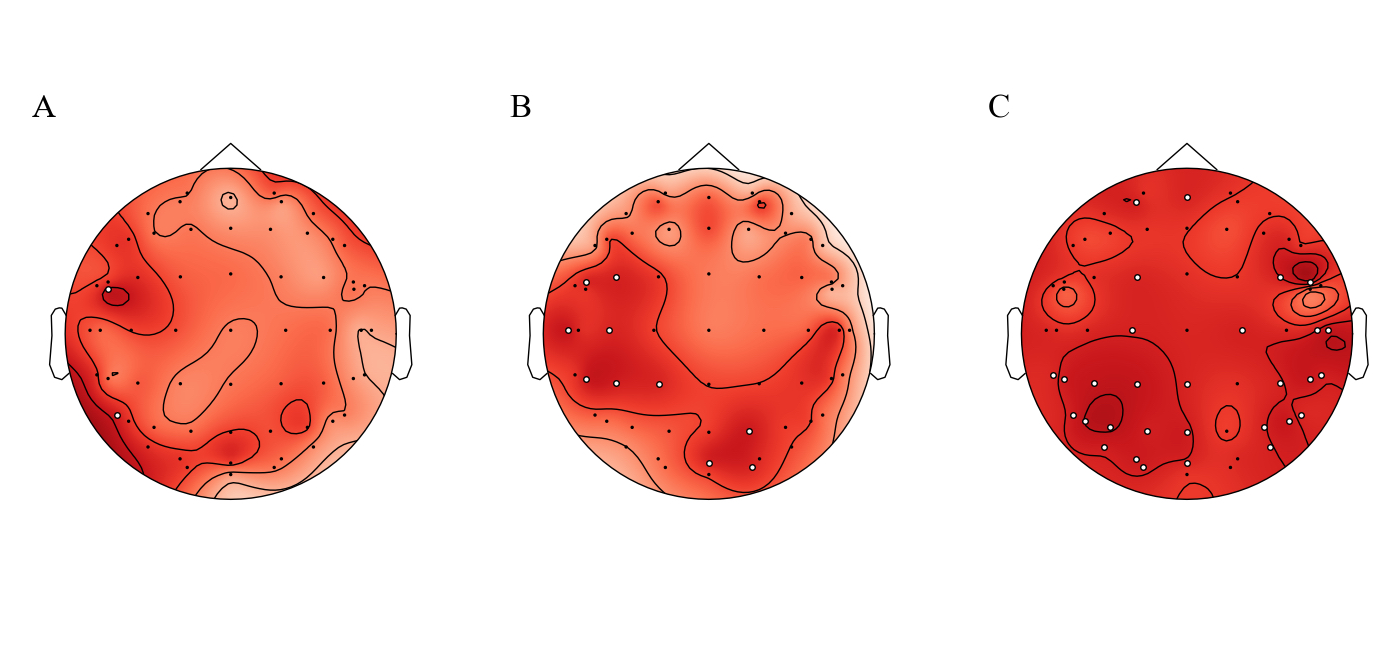
\includegraphics[width=0.9\linewidth]{figures/topographic}
  \caption[Topographic Analysis of \tvt Accuracy]{
    The results of the model on various brain regions. Each sensor represents a 
    group containing it and its immediate neighbors, and we calculated \tvt 
    accuracy using single groups.  A topographic plot of the \tvt accuracies is 
    shown for three time periods: {\bf A}  0--500ms window; {\bf B} 0ms--1000ms 
    window; and {\bf C} 0--1000ms window. Statistically significant groups are 
    shown in white ($p < 0.001$, FDR corrected).
  }
  \label{fig:topographic}
\end{figure}

In this experiment we test which areas of the brain are contributing the most 
to the \tvt accuracy. We categorized sensors into $n_s$ groups for analysis, 
where each group consists of a primary sensor and its neighboring sensors. We 
used the accuracy of each sensor group to annotate the accuracy of the primary 
sensor, and then performed a topographic interpolation of the \tvt accuracy 
over the brain. 

The topographic interpolation of three time windows is visible in 
Figure~\ref{fig:topographic}. We see lower \tvt accuracies for the earlier time 
window (0-500ms) compared to the later time window (500ms-1000ms), however we 
see the highest accuracies over the entire time window (0-1000ms). Removing a 
substantial amount of data effects accuracy negatively, however a large amount 
of the sensors remain statistically significance, which indicates that the 
semantic representation is highly distributed across the cortex.
